\begin{frame}{Anatomy of an Enterprise Copilot}

  {\centering
  \resizebox{\textwidth}{!}{%
  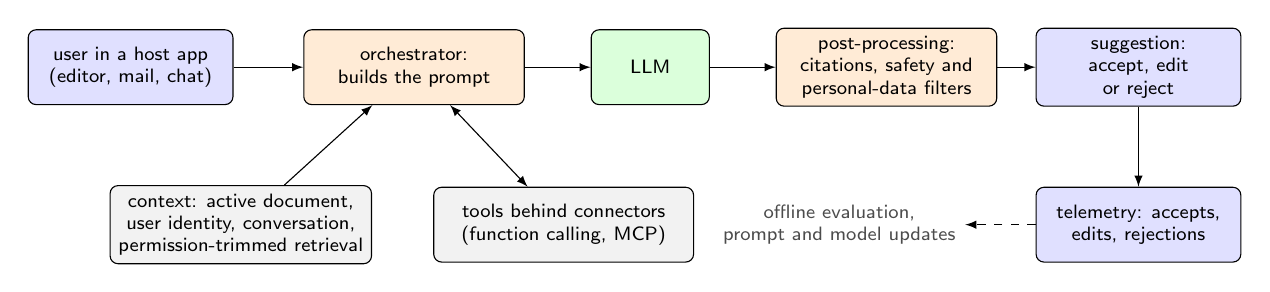
\begin{tikzpicture}[font=\sffamily\scriptsize, >=latex,
      box/.style={draw, rounded corners=0.1cm, align=center, minimum height=0.95cm, inner sep=3pt},
      app/.style={box, fill=blue!12, minimum width=2.6cm},
      orch/.style={box, fill=orange!16, minimum width=2.8cm},
      llm/.style={box, fill=green!14, minimum width=1.5cm},
      src/.style={box, fill=gray!10, minimum width=3.3cm},
      note/.style={align=center, text=black!70}]
    \node[app]  (app)  at (0,2.2)    {user in a host app\\(editor, mail, chat)};
    \node[orch] (orc)  at (3.6,2.2)  {orchestrator:\\builds the prompt};
    \node[llm]  (llm)  at (6.6,2.2)  {LLM};
    \node[orch] (post) at (9.6,2.2)  {post-processing:\\citations, safety and\\personal-data filters};
    \node[app]  (sug)  at (12.8,2.2) {suggestion:\\accept, edit\\or reject};
    \node[src]  (ctx)  at (1.4,0.2)  {context: active document,\\user identity, conversation,\\permission-trimmed retrieval};
    \node[src]  (tool) at (5.5,0.2)  {tools behind connectors\\(function calling, MCP)};
    \node[app]  (tel)  at (12.8,0.2) {telemetry: accepts,\\edits, rejections};
    \draw[->] (app) -- (orc);
    \draw[->] (orc) -- (llm);
    \draw[->] (llm) -- (post);
    \draw[->] (post) -- (sug);
    \draw[->] (ctx) -- (orc);
    \draw[<->] (orc) -- (tool);
    \draw[->] (sug) -- (tel);
    \draw[->, dashed] (tel.west) -- (10.6,0.2) node[note, anchor=east] {offline evaluation,\\prompt and model updates};
  \end{tikzpicture}}\\[0.3em]
  {\scriptsize One request runs along the top row. The dashed arrow is the slow loop: logged outcomes feed evaluation and later updates.\par}\par}
  \vspace{0.2em}
  \begin{itemize}\footnotesize\itemsep0.3em
    \item[\textcolor{red}{$\blacktriangleright$}] \textbf{Copilot:} an assistant inside a tool the person already uses. It proposes a draft, an answer or an edit; the person accepts, edits or rejects it and stays responsible for the result. An agent (covered earlier) carries out multi-step actions itself.
    \item[\textcolor{red}{$\blacktriangleright$}] \textbf{Orchestrator:} the service between the app and the model. It builds the prompt, calls the model, executes the tool calls the model emits, and filters the output. GitHub Copilot's prompt assembly for code completion (covered earlier) is a small instance.
    \item[\textcolor{red}{$\blacktriangleright$}] \textbf{Grounding:} adding retrieved organisational content to the prompt at request time, so the answer can cite it. Retrieval runs with the asking user's permissions (see the scalable RAG section of this lecture).
  \end{itemize}
\end{frame}

\begin{frame}{Field Evidence on Copilot Productivity}

  {\centering\scriptsize
  \begin{tabular}{>{\raggedright\arraybackslash}p{2.4cm} >{\raggedright\arraybackslash}p{4.0cm} >{\raggedright\arraybackslash}p{5.6cm}}
    \toprule
    \textbf{Study} & \textbf{Setting and design} & \textbf{Measured effect} \\
    \midrule
    Peng et al.\ 2023 (covered earlier) & one timed task (an HTTP server in JavaScript), randomised & 55.8\% faster \\
    \addlinespace[0.2em]
    Brynjolfsson, Li, Raymond, QJE 2025 & 5{,}172 customer-support agents; GPT-based reply suggestions; staggered roll-out & +15\% issues resolved per hour; about +30\% for less skilled and less experienced agents; small quality losses for the most skilled \\
    \addlinespace[0.2em]
    Cui et al., Management Science 2026 & three randomised field experiments; 4{,}867 developers; GitHub Copilot & +26.08\% completed tasks (standard error 10.3 points); larger gains for less experienced developers \\
    \addlinespace[0.2em]
    Becker et al.\ (METR) 2025 & randomised; 16 developers, 246 tasks in repositories they knew (5 years on average) & tasks took 19\% longer when AI tools were allowed \\
    \bottomrule
  \end{tabular}\par}
  \vspace{0.4em}
  \begin{itemize}\scriptsize\itemsep0.3em
    \item[\textcolor{red}{$\blacktriangleright$}] \textbf{The sign depends on the setting.} Gains concentrate in less experienced workers; experienced developers in large codebases they knew well were slowed down. METR's results are ``consistent with small greenfield projects or development in unfamiliar codebases seeing substantial speedup''.
    \item[\textcolor{red}{$\blacktriangleright$}] \textbf{Field estimates are wide.} Even over 4{,}867 developers, $26.08 \pm 1.96 \times 10.3$ gives a 95\% interval of about 6\% to 46\%; decide a roll-out with a randomised comparison on your own tasks.
  \end{itemize}
  \vspace{0.1em}
  {\scriptsize Brynjolfsson, Li, Raymond, ``Generative AI at Work,'' \textit{QJE} 140(2), 2025, \href{https://doi.org/10.1093/qje/qjae044}{doi:10.1093/qje/qjae044} (figures: \href{https://arxiv.org/abs/2304.11771v2}{arXiv:2304.11771v2}); Cui et al., \textit{Management Science}, 2026, \href{https://doi.org/10.1287/mnsc.2025.00535}{doi:10.1287/mnsc.2025.00535}; Becker et al.\ (METR), \href{https://arxiv.org/abs/2507.09089v2}{arXiv:2507.09089v2}.\par}
\end{frame}

\begin{frame}{Perceived Versus Measured Speed-Up}
  \begin{columns}[T,onlytextwidth]
    \column{0.50\textwidth}
      \begin{itemize}\scriptsize\itemsep0.35em
        \item[\textcolor{red}{$\blacktriangleright$}] \textbf{Forecasts and self-reports missed the sign.} METR's developers forecast that AI would cut their completion time by 24\%, and afterwards believed it had cut it by 20\%; measured, it rose by 19\%. Economics and ML experts had predicted cuts of 39\% and 38\%.
        \item[\textcolor{red}{$\blacktriangleright$}] \textbf{Acceptance rate:} the fraction of shown completions that the developer accepts. Over 2{,}631 survey responses from GitHub Copilot users, it predicted perceived productivity (Pearson 0.24) better than whether accepted code persisted; Copilot's rate was 27\%.
        \item[\textcolor{red}{$\blacktriangleright$}] \textbf{It can be gamed.} The authors note that splitting each suggestion in two would likely raise the rate without helping the user (Goodhart's law, covered earlier).
        \item[\textcolor{red}{$\blacktriangleright$}] \textbf{Rule:} monitor with telemetry; decide with a randomised control group on your own tasks.
      \end{itemize}
    \column{0.48\textwidth}
      \centering
      \vspace{0.6em}
      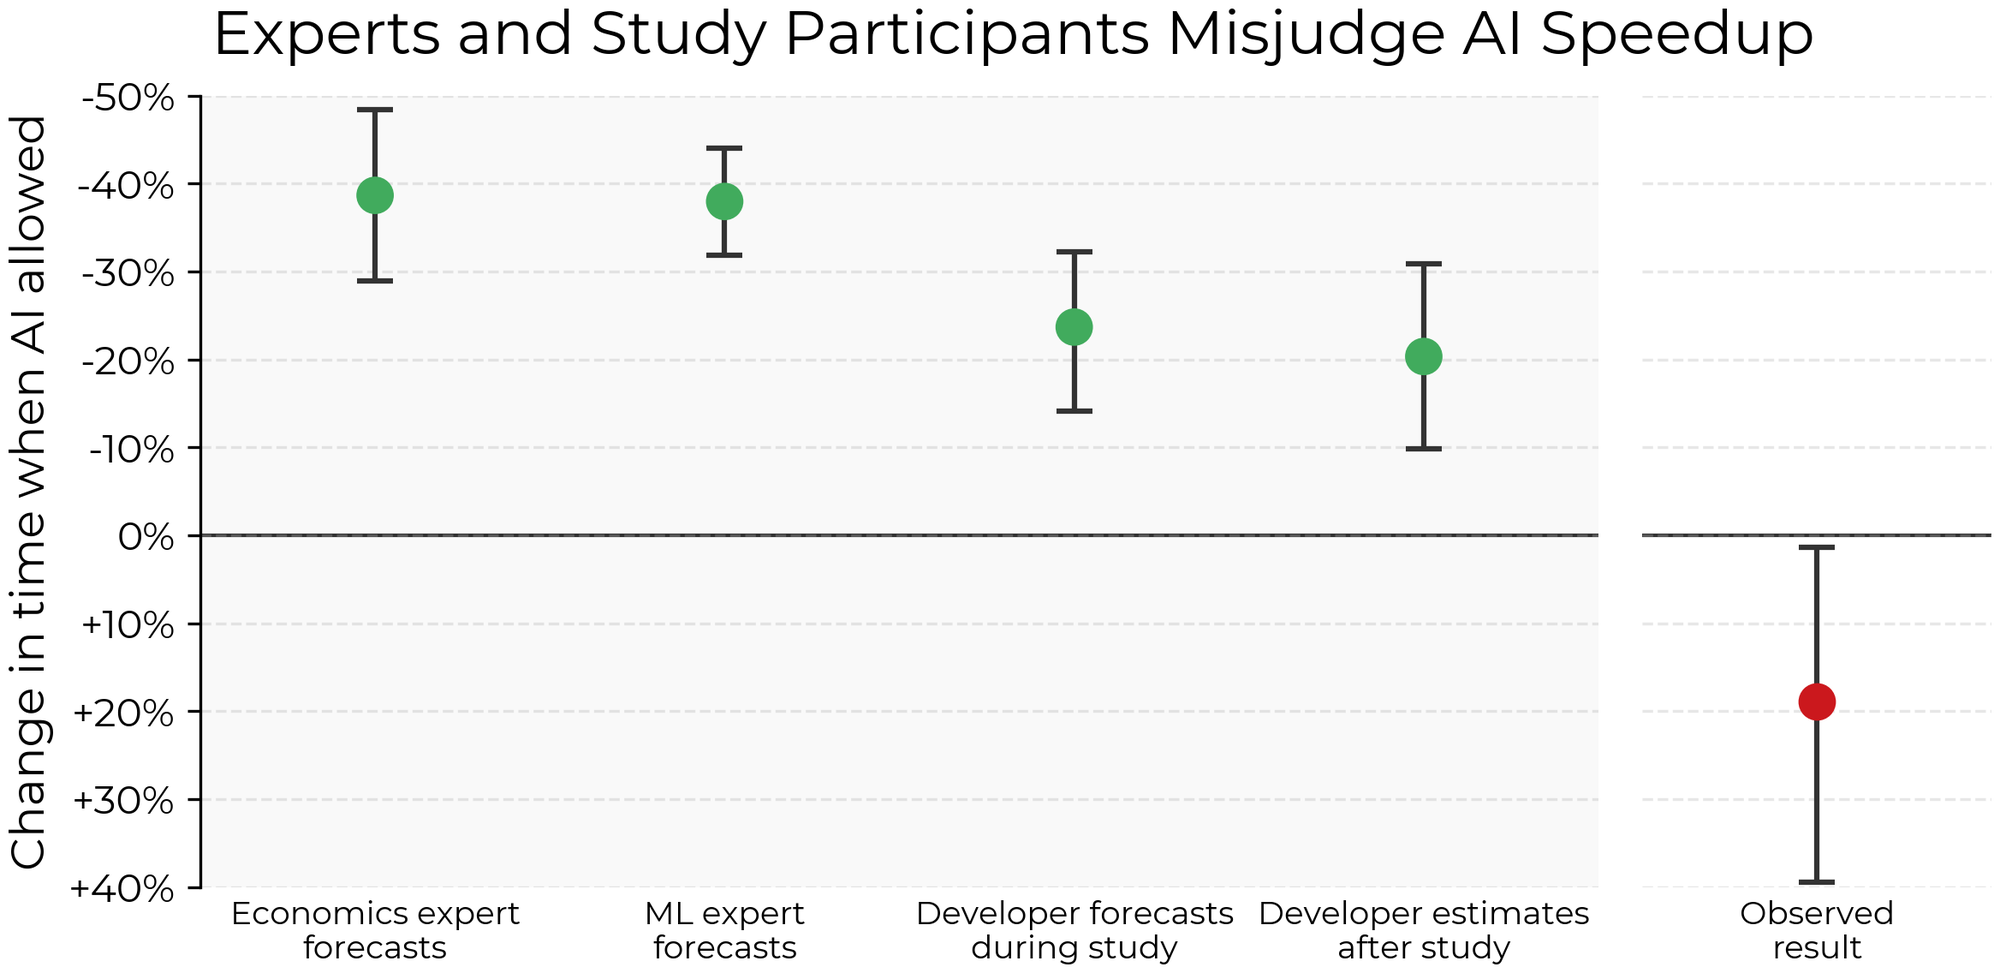
\includegraphics[width=\linewidth,height=0.5\textheight,keepaspectratio]{images/nlp-security-enterprise/metr_fig1_forecast_vs_observed.png}\\[0.2em]
      {\scriptsize Becker et al., ``Measuring the Impact of Early-2025 AI on Experienced Open-Source Developer Productivity,'' \href{https://arxiv.org/abs/2507.09089v2}{arXiv:2507.09089v2}, Figure~1.\par}
  \end{columns}
  \vspace{0.1em}
  {\scriptsize Ziegler et al., ``Productivity Assessment of Neural Code Completion,'' MAPS 2022, \href{https://arxiv.org/abs/2205.06537v1}{arXiv:2205.06537v1}.}
\end{frame}

\begin{frame}{Oversharing: A Copilot Inherits Every Permission}
  \begin{columns}[T,onlytextwidth]
    \column{0.55\textwidth}
      \begin{itemize}\scriptsize\itemsep0.45em
        \item[\textcolor{red}{$\blacktriangleright$}] \textbf{Oversharing:} access that is broader than the content's owner intends, such as a site shared with the whole organisation or a link anyone can open. Permission-aware retrieval (see the scalable RAG section of this lecture) enforces the permissions it is given, careless ones included.
        \item[\textcolor{red}{$\blacktriangleright$}] An overshared file used to stay unseen because nobody searched for it. A copilot searches everything the user can open, so one ordinary question can surface it, with a citation.
        \item[\textcolor{red}{$\blacktriangleright$}] Microsoft's documentation states both halves: ``Microsoft Copilot only surfaces organizational data to which individual users have at least view permissions'' and ``By default, SharePoint sets sharing settings to the most permissive option''.
        \item[\textcolor{red}{$\blacktriangleright$}] \textbf{Clean up before the roll-out:} report sites shared organisation-wide or through broad links; review access per site and per user; hide high-risk sites from copilot retrieval while they are fixed, leaving permissions unchanged; make new links narrow and expiring.
      \end{itemize}
    \column{0.43\textwidth}
      \centering
      \vspace{0.8em}
      \begin{tikzpicture}[font=\sffamily\scriptsize, >=latex, scale=0.9, every node/.style={transform shape}]
        \fill[red!10] (0,0) ellipse (2.7cm and 1.75cm);
        \draw[thick] (0,0) ellipse (2.7cm and 1.75cm);
        \fill[green!20] (-0.75,-0.15) ellipse (1.3cm and 0.85cm);
        \draw (-0.75,-0.15) ellipse (1.3cm and 0.85cm);
        \node[align=center] at (-0.75,-0.15) {what this user\\should see};
        \node[align=center, text=KAred] at (1.55,0.25) {overshared:\\can open,\\should not};
        \node[align=center] at (0,2.1) {everything this user can open};
        \draw[->, thick, KAUSTblue] (0,-2.5) -- (0,-1.8);
        \node[align=center] at (0,-2.8) {copilot retrieval searches all of it};
      \end{tikzpicture}\\[0.3em]
      {\scriptsize Permission-aware retrieval stops at the outer boundary. Only the inner region was meant for this user.\par}
  \end{columns}
  \vspace{0.2em}
  {\scriptsize Microsoft Learn, ``Data, Privacy, and Security for Microsoft Copilot,'' 2026, \href{https://learn.microsoft.com/en-us/microsoft-365/copilot/microsoft-365-copilot-privacy}{learn.microsoft.com}; ``Get ready for Microsoft Copilot with SharePoint Advanced Management,'' 2026, \href{https://learn.microsoft.com/en-us/microsoft-365/copilot/get-ready-copilot-sharepoint-advanced-management}{learn.microsoft.com}.}
\end{frame}

\begin{frame}{EchoLeak: Zero-Click Exfiltration From a Copilot}

  {\centering
  \resizebox{\textwidth}{!}{%
  \begin{tikzpicture}[font=\sffamily\scriptsize, >=latex,
      stage/.style={draw, rounded corners=0.1cm, align=left, text width=3.2cm, minimum height=1.5cm, fill=orange!14, inner sep=3pt},
      byp/.style={align=left, text width=3.2cm, text=KAred, anchor=north}]
    \node[stage] (s1) at (0,0)    {\textbf{1. Email in.} The attacker mails the victim; the instructions read as advice to the human and never mention AI.};
    \node[stage] (s2) at (3.65,0) {\textbf{2. Retrieved.} The victim asks Copilot an ordinary question; retrieval puts a chunk of the email into context.};
    \node[stage] (s3) at (7.3,0)  {\textbf{3. Data packed.} The model copies ``THE MOST sensitive'' data in context into a Markdown image URL.};
    \node[stage] (s4) at (10.95,0) {\textbf{4. Data out.} The client loads the image through an allow-listed Teams URL, which fetches the attacker's server.};
    \draw[->] (s1) -- (s2);
    \draw[->] (s2) -- (s3);
    \draw[->] (s3) -- (s4);
    \node[byp] at (0,-0.95)    {passes the XPIA (cross-prompt injection attack) classifier};
    \node[byp] at (3.65,-0.95) {``RAG spraying'': many topic headings, so many questions retrieve it};
    \node[byp] at (7.3,-0.95)  {reference-style \texttt{![alt][ref]} escapes link and image redaction};
    \node[byp] at (10.95,-0.95) {passes the page's Content Security Policy (CSP) allowlist; zero clicks};
  \end{tikzpicture}}\par}
  \vspace{0.1em}
  \begin{itemize}\scriptsize\itemsep0.25em
    \item[\textcolor{red}{$\blacktriangleright$}] \textbf{EchoLeak} (tracked as CVE-2025-32711) was \textbf{zero-click}: the victim does nothing beyond normal use, and ``an adversary simply needs to send an email to the victim''. Microsoft rated it critical (9.3 of 10) and had fixed it server-side when Aim Security disclosed it on 11 June 2025.
    \item[\textcolor{red}{$\blacktriangleright$}] \textbf{All three legs of the lethal trifecta} (covered earlier): private data in context, an untrusted email retrieved like any internal file, and an outbound channel the client opens by itself. Aim Security calls this an LLM scope violation: untrusted input steers the model to trusted data without the user's consent.
    \item[\textcolor{red}{$\blacktriangleright$}] \textbf{Defenses named in the sources:} leave external email out of answers about internal data unless the user asks (Microsoft's label-based exclusions, at a cost in capability); render only an allowlisted Markdown subset, stripping external links and images in every syntax; allow only the origins the page needs, with no wildcards; treat injection classifiers as one layer (jailbreak defenses section).
  \end{itemize}
  \vspace{0.1em}
  {\scriptsize Chain as described in Aim Security's EchoLeak write-up, 11 June 2025, \href{https://web.archive.org/web/20250612074812/https://www.aim.security/lp/aim-labs-echoleak-blogpost}{aim.security (archived)}; Microsoft Security Response Center, \href{https://msrc.microsoft.com/update-guide/vulnerability/CVE-2025-32711}{CVE-2025-32711}; Reddy and Gujral, AAAI Fall Symposium 2025, \href{https://arxiv.org/abs/2509.10540v1}{arXiv:2509.10540v1}.}
\end{frame}
